\section{Pilot Study}
\label{sec:pilot}

Our pilot study uses CRIT, and it aims to answer two questions:
Should all prompts be issued to GPT-3 sequentially or they
can be issued all together?  
What limitations can be identified for improvement?
The study utilizes exercises with established answers from the $8^{th}$ edition of the textbook ``Ask the Right Questions'' by the authors of \cite{AskRightQ2001}. It is important to note that the study evaluates the effectiveness of CRIT's prompt template, rather than the language models to which CRIT can issue prompts.

\begin{comment}
Table~\ref{tab:pilot1} presents two examples from \cite{AskRightQ2001}. The results of the CRIT analysis, which include conclusion extraction and reason identification, match or exceed the evaluations made by the authors. In the first example, the authors consider the document to be somewhat ambiguous with two potential conclusions. CRIT finds the document to be poorly written without a clear conclusion and gives it a low validity score of $60\%$. This low credibility score is attributed to the absence of sufficient evidence in the argument to justify two possible claims. 
In the second example, CRIT accurately extracts the claim and arguments and recognizes that the argument's validity is subjective and dependent on context such as religious beliefs and cultural perspectives. 
\end{comment}

On short documents, the results are similar in quality when CRIT is used to issue prompts either sequentially or all together as one prompt, as long as the instructions are consistent. However, when evaluating long articles in \cite{501Q2004}, CRIT issuing prompts one after another yields much higher presentation quality in both organization and clarity. 
(Due to the space limit, we document examples in a supplement document \cite{CRITExtended2023}.) In the teaching mode, the sequential option is thus much preferred. Furthermore,
When a reason is itself a claim and requires CRIT to validate its supporting references, using a sequential approach is more flexible and enables CRIT to query for references and then execute the process recursively.

\begin{table}[hbt!]
%\vspace{-.1in}
%\resizebox{\textwidth}{!}
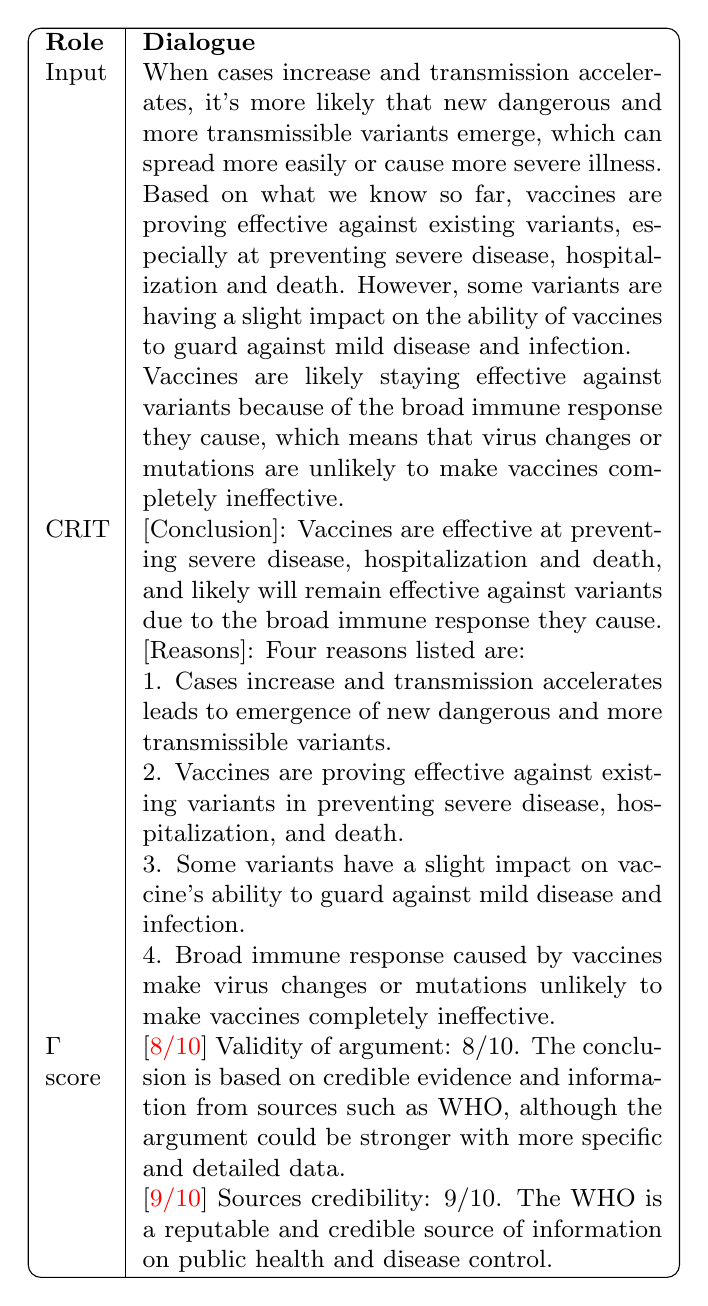
\begin{tikzpicture}
\begin{small}
\node (table) [inner sep=0pt] {
\begin{tabular}{p{0.8cm}|p{6.6cm}}
\toprule
\textbf{Role} & \textbf{Dialogue} \\
\midrule
{Input} & {When cases increase and transmission accelerates, it’s more likely that new dangerous and more transmissible variants emerge, which can spread more easily or cause more severe illness.

Based on what we know so far, vaccines are proving effective against existing variants, especially at preventing severe disease, hospitalization and death. However, some variants are having a slight impact on the ability of vaccines to guard against mild disease and infection.

Vaccines are likely staying effective against variants because of the broad immune response they cause, which means that virus changes or mutations are unlikely to make vaccines completely ineffective.} \\

{CRIT} & {[Conclusion]: Vaccines are effective at preventing severe disease, hospitalization and death, and likely will remain effective against variants due to the broad immune response they cause.} \\

& [Reasons]: Four reasons listed are: \\
& 1.  Cases increase and transmission accelerates leads to emergence of new dangerous and more transmissible variants. \\
& 2. Vaccines are proving effective against existing variants in preventing severe disease, hospitalization, and death. \\
& 3. Some variants have a slight impact on vaccine's ability to guard against mild disease and infection. \\
& 4. Broad immune response caused by vaccines make virus changes or mutations unlikely to make vaccines completely ineffective. \\
\midrule
{$\Gamma$ score} & {[{\color{red}8/10}] Validity of argument: 8/10. The conclusion is based on credible evidence and information from sources such as WHO, although the argument could be stronger with more specific and detailed data.} \\
& {[{\color{red}9/10}] Sources credibility: 9/10. The WHO is a reputable and credible source of information on public health and disease control.} \\
%\textbf{Final Score}: {\color{red}$72\%$ High} (High: above $60\%$, Low: below $25\%$)
%$} \\
\bottomrule
\end{tabular}
};
\draw [rounded corners=.5em] (table.north west) rectangle (table.south east);
\end{small}
\end{tikzpicture}
%\vspace{-.05in}
\caption{Pilot Study on CRIT. 
%WHO's post about the expected efficacy of 
%COVID vaccines on its variants.
}
\vspace{-.20in}
\label{tab:pilot2}
\end{table}

Table~\ref{tab:pilot2} presents a document about COVID-19 vaccine efficacy, published by the World Health Organization (WHO) in July 2021 on its homepage \cite{WHO2021}. The article remains available on the WHO's website, indicating that its information is still considered valid by the organization. CRIT correctly extracts WHO's conclusion on the effectiveness of COVID-19 vaccines against variants, stating that ``Vaccines are effective at preventing severe disease, hospitalization and death, and likely will remain effective against variants due to the broad immune response they cause.'' This conclusion is supported by four strong arguments. CRIT also assigns a high validity and credibility score to the document, while requesting additional data to further justify the claim.



